\begin{figure}[t]
\centering
	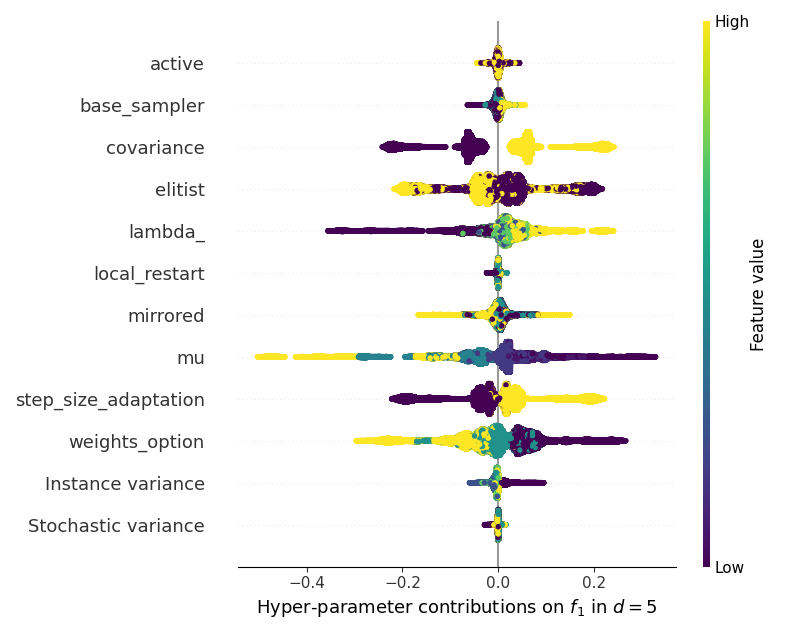
\includegraphics[height=0.15\textheight,trim=0mm 0mm 30mm 0mm,clip]{cma_img_new/img_summary_f1_d5.png}
	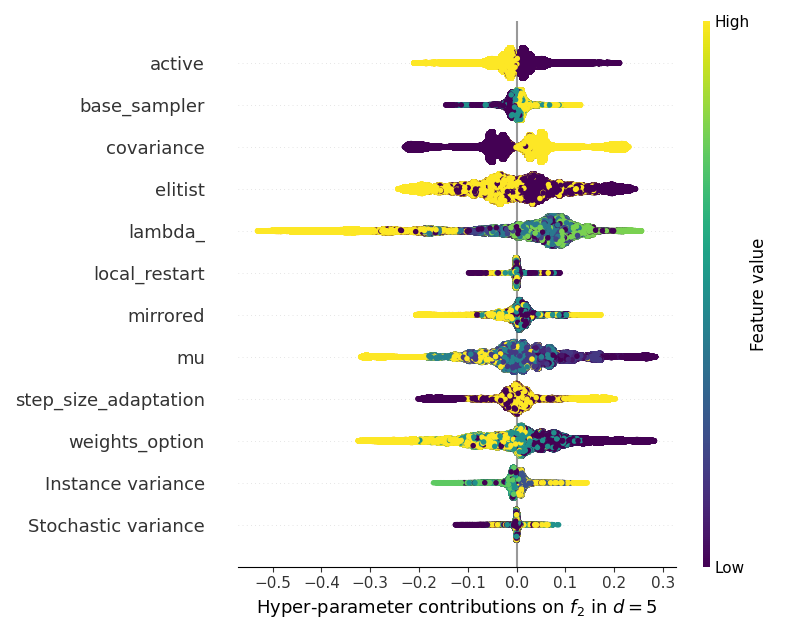
\includegraphics[height=0.15\textheight,trim=60mm 0mm 30mm 0mm,clip]{cma_img_new/img_summary_f2_d5.png}
	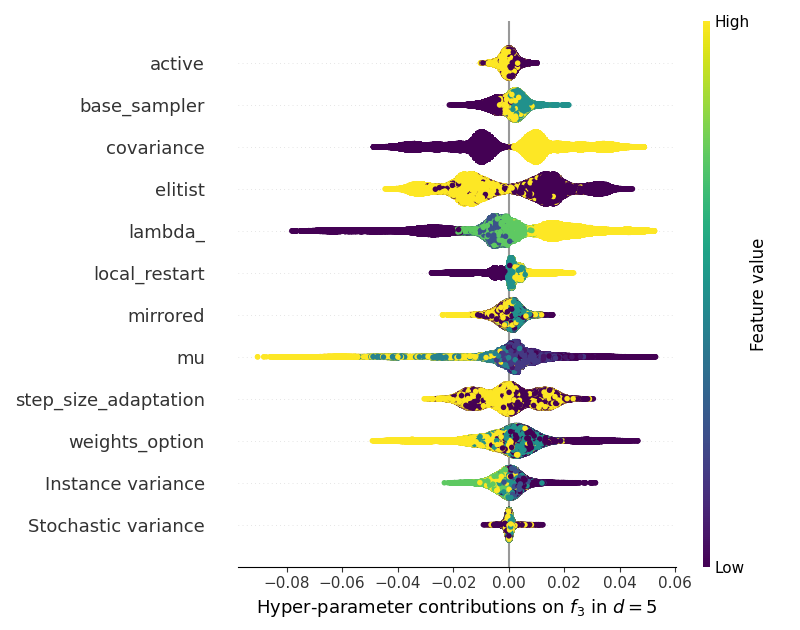
\includegraphics[height=0.15\textheight,trim=60mm 0mm 30mm 0mm,clip]{cma_img_new/img_summary_f3_d5.png}
	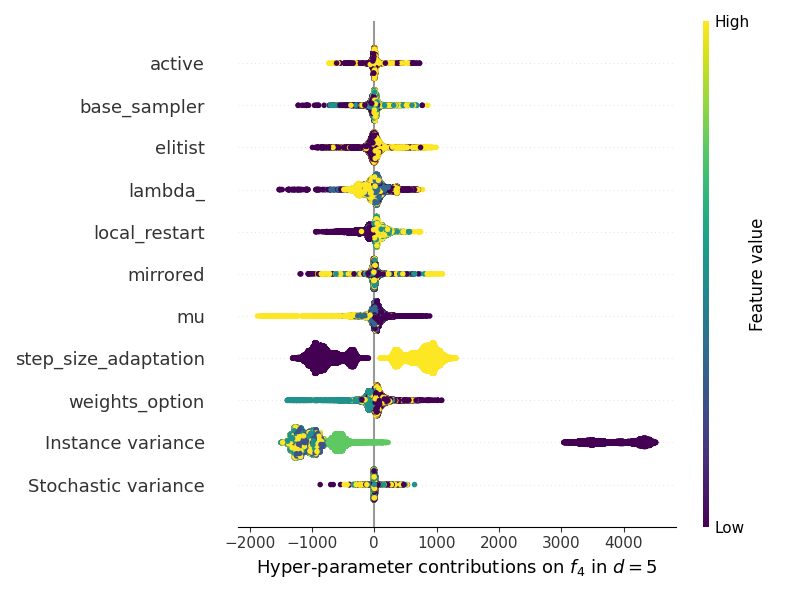
\includegraphics[height=0.15\textheight,trim=60mm 0mm 0mm 0mm,clip]{cma_img_new/img_summary_f4_d5.png}
	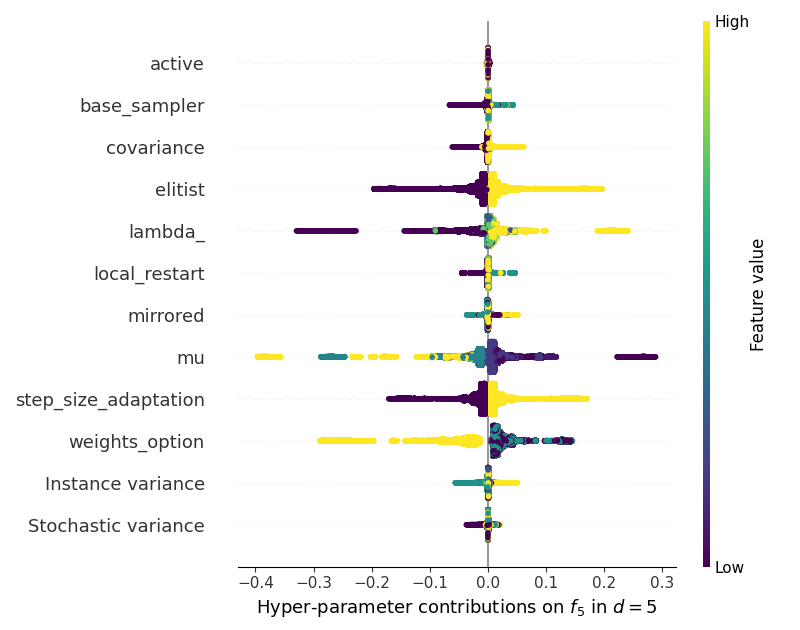
\includegraphics[height=0.15\textheight,trim=0mm 0mm 30mm 0mm,clip]{cma_img_new/img_summary_f5_d5.png}
	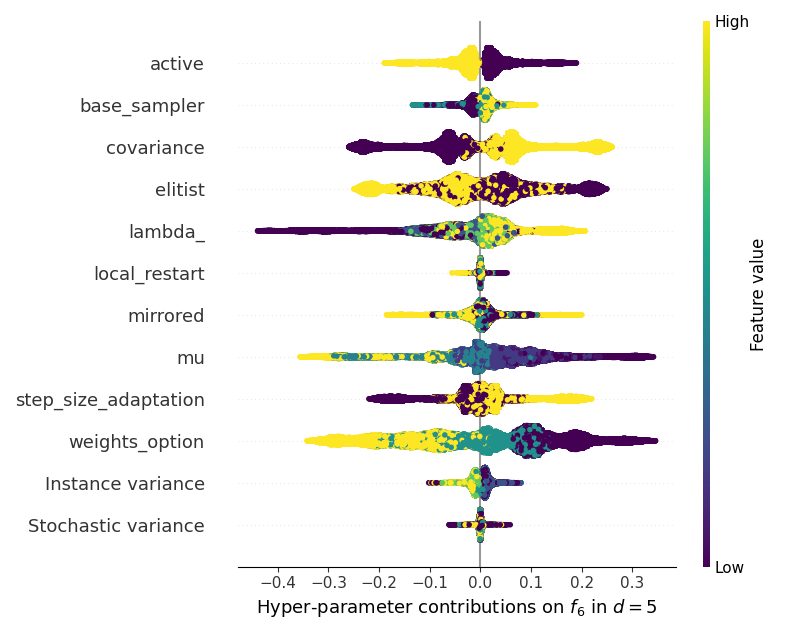
\includegraphics[height=0.15\textheight,trim=60mm 0mm 30mm 0mm,clip]{cma_img_new/img_summary_f6_d5.png}
	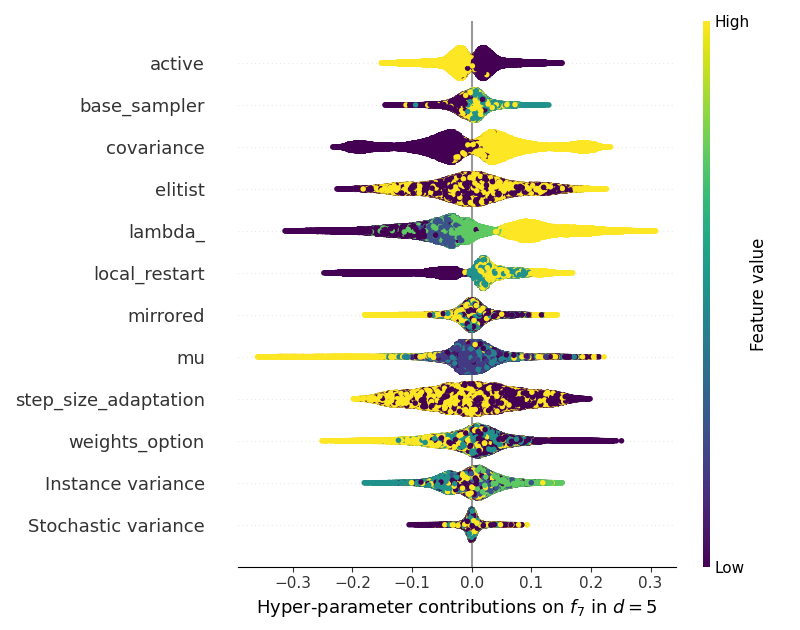
\includegraphics[height=0.15\textheight,trim=60mm 0mm 30mm 0mm,clip]{cma_img_new/img_summary_f7_d5.png}
	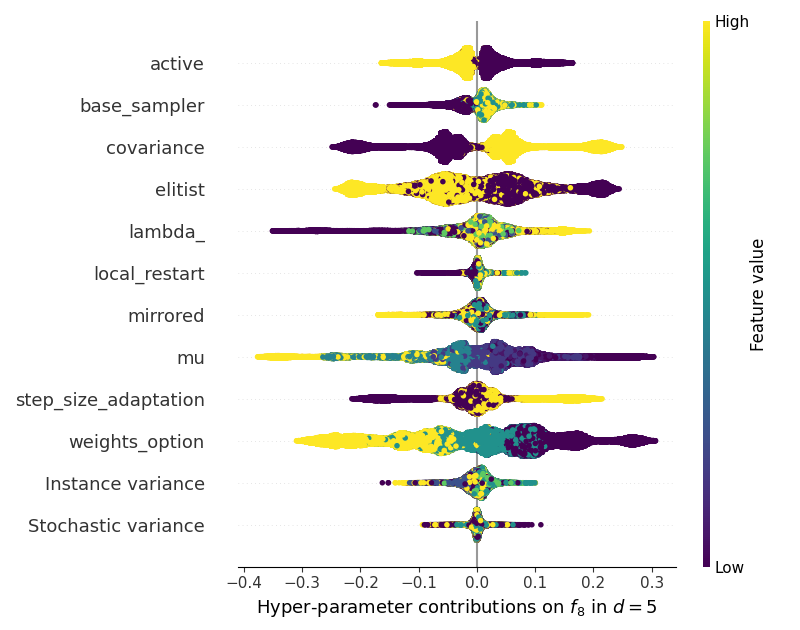
\includegraphics[height=0.15\textheight,trim=60mm 0mm 0mm 0mm,clip]{cma_img_new/img_summary_f8_d5.png}
	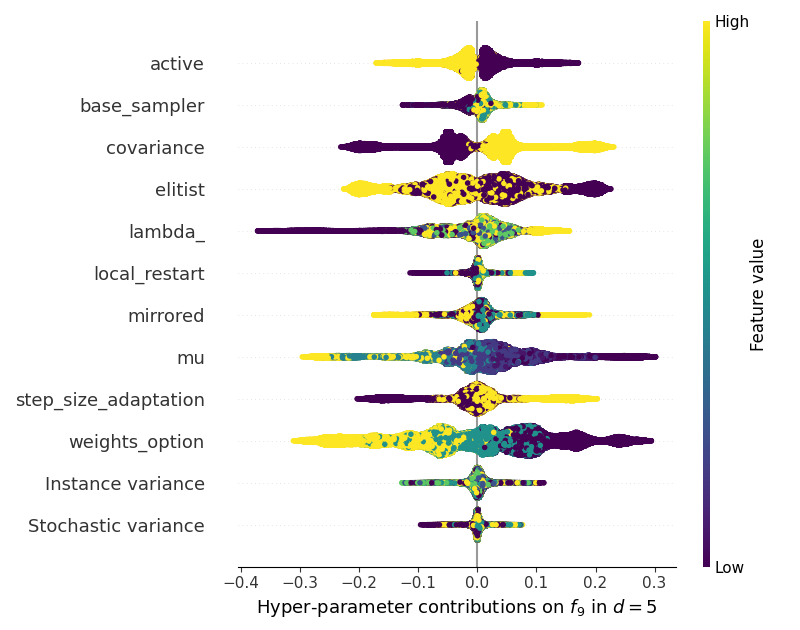
\includegraphics[height=0.15\textheight,trim=0mm 0mm 30mm 0mm,clip]{cma_img_new/img_summary_f9_d5.png}
	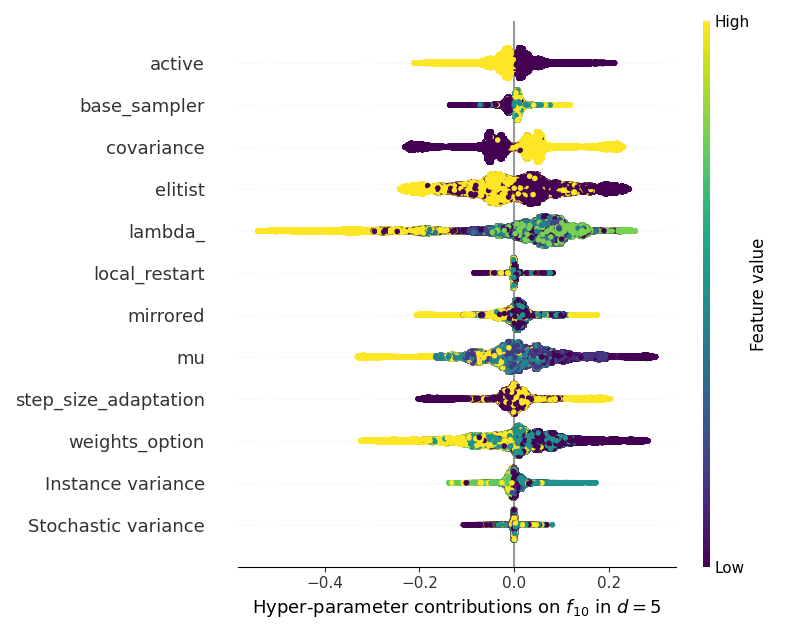
\includegraphics[height=0.15\textheight,trim=60mm 0mm 30mm 0mm,clip]{cma_img_new/img_summary_f10_d5.png}
	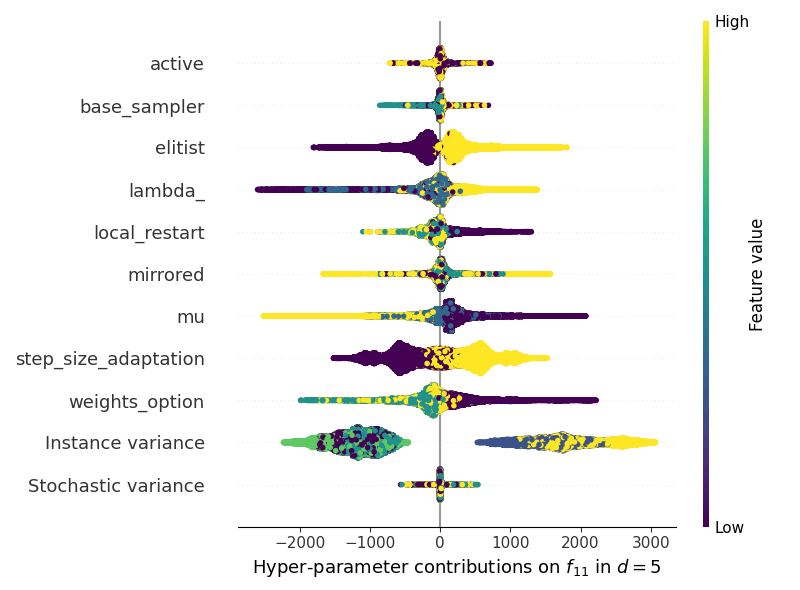
\includegraphics[height=0.15\textheight,trim=60mm 0mm 30mm 0mm,clip]{cma_img_new/img_summary_f11_d5.png}
	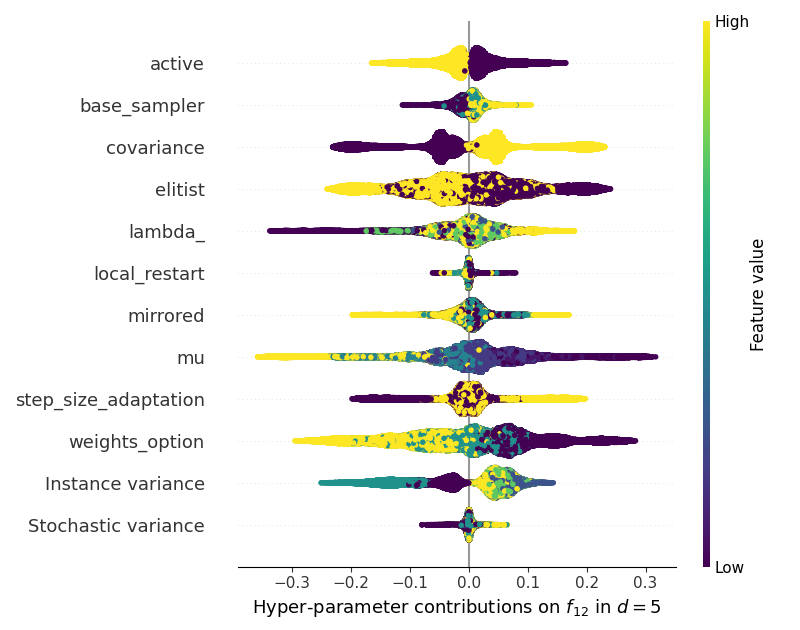
\includegraphics[height=0.15\textheight,trim=60mm 0mm 0mm 0mm,clip]{cma_img_new/img_summary_f12_d5.png}
	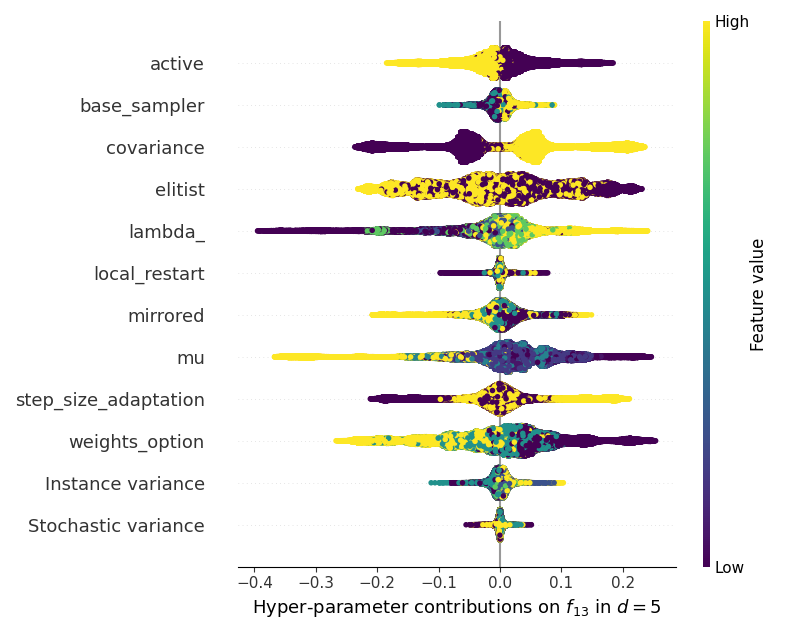
\includegraphics[height=0.15\textheight,trim=0mm 0mm 30mm 0mm,clip]{cma_img_new/img_summary_f13_d5.png}
	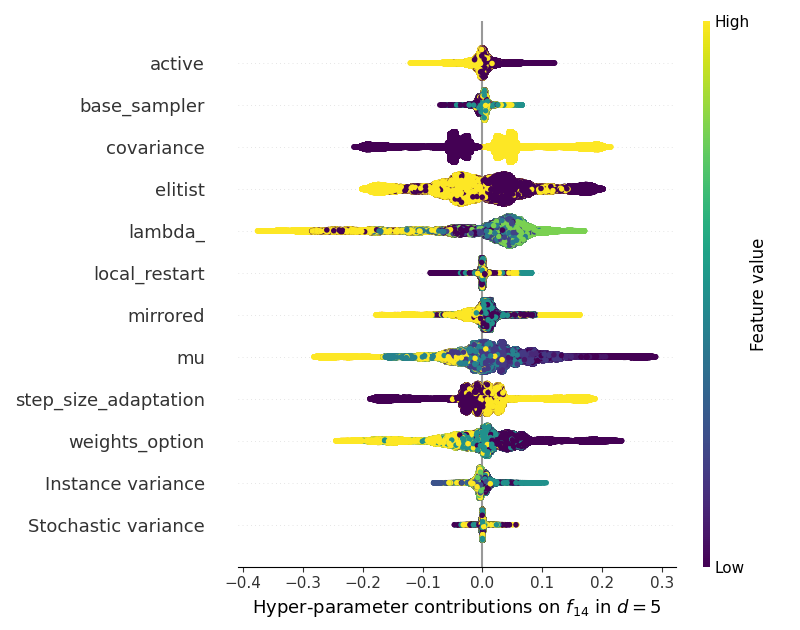
\includegraphics[height=0.15\textheight,trim=60mm 0mm 30mm 0mm,clip]{cma_img_new/img_summary_f14_d5.png}
	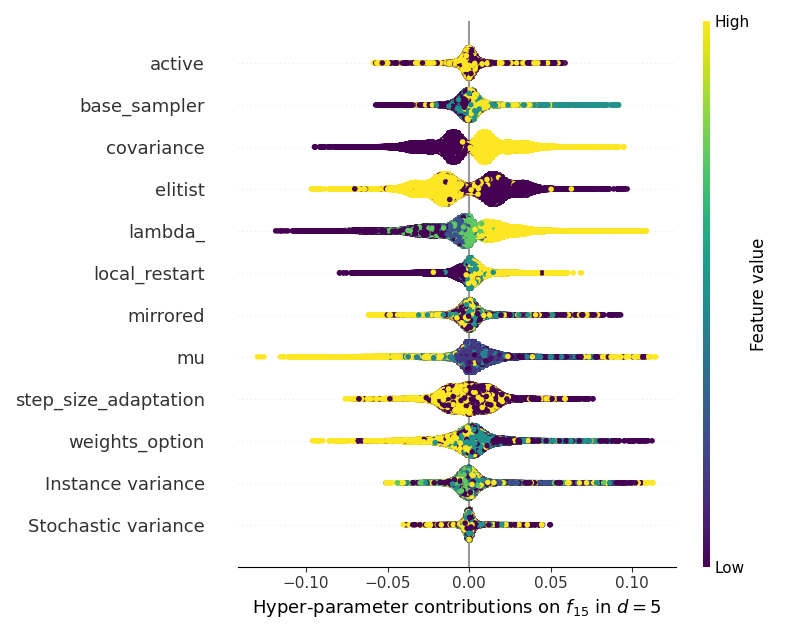
\includegraphics[height=0.15\textheight,trim=60mm 0mm 30mm 0mm,clip]{cma_img_new/img_summary_f15_d5.png}
	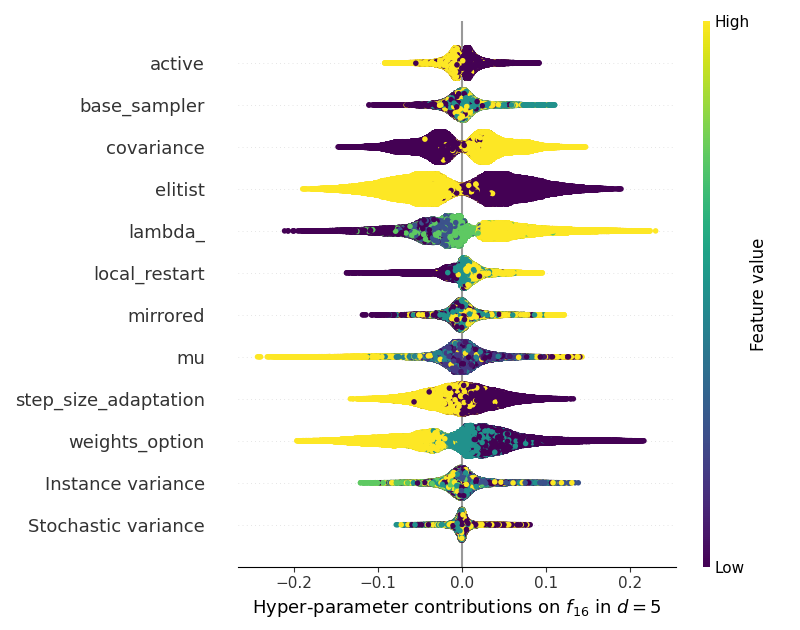
\includegraphics[height=0.15\textheight,trim=60mm 0mm 0mm 0mm,clip]{cma_img_new/img_summary_f16_d5.png}
	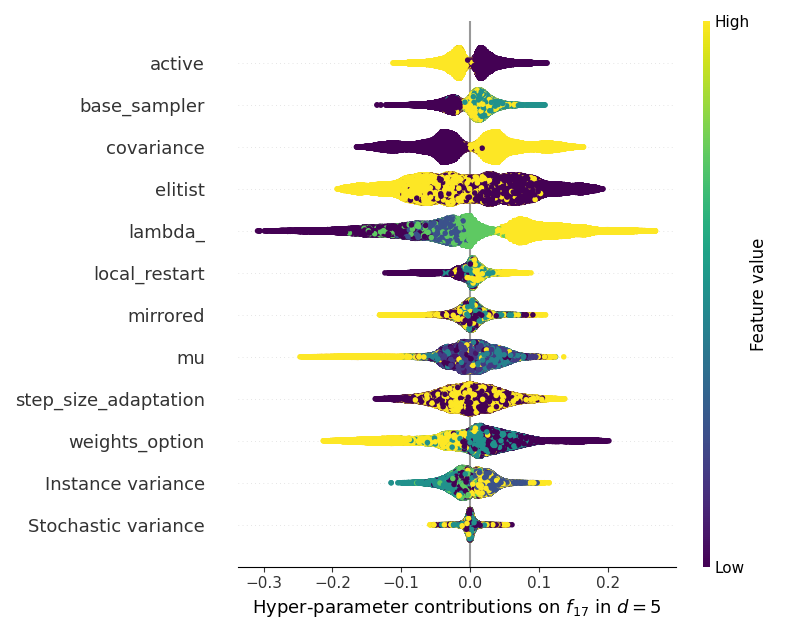
\includegraphics[height=0.15\textheight,trim=0mm 0mm 30mm 0mm,clip]{cma_img_new/img_summary_f17_d5.png}
	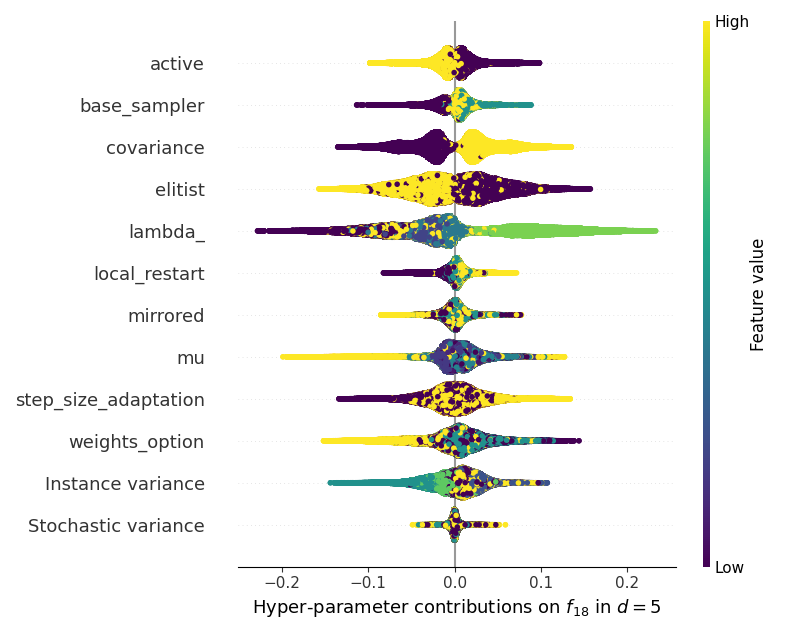
\includegraphics[height=0.15\textheight,trim=60mm 0mm 30mm 0mm,clip]{cma_img_new/img_summary_f18_d5.png}
	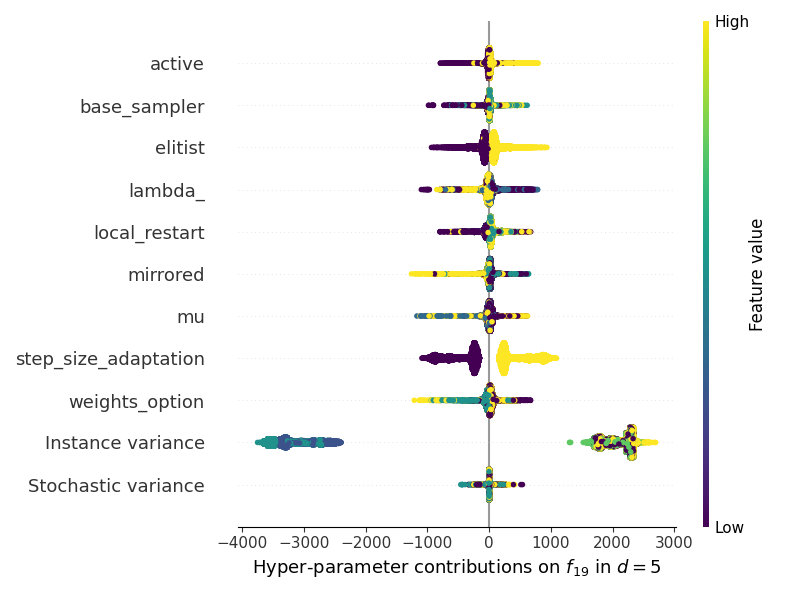
\includegraphics[height=0.15\textheight,trim=60mm 0mm 30mm 0mm,clip]{cma_img_new/img_summary_f19_d5.png}
	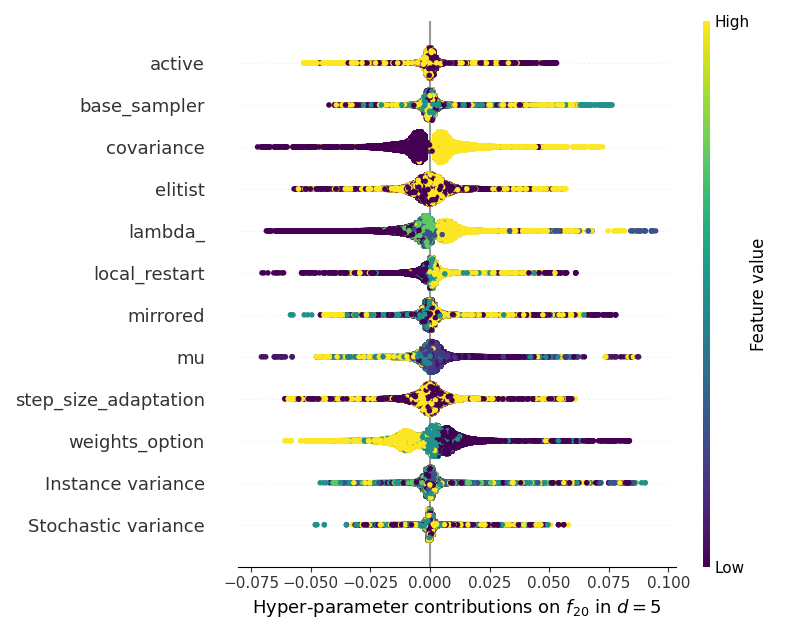
\includegraphics[height=0.15\textheight,trim=60mm 0mm 0mm 0mm,clip]{cma_img_new/img_summary_f20_d5.png}
	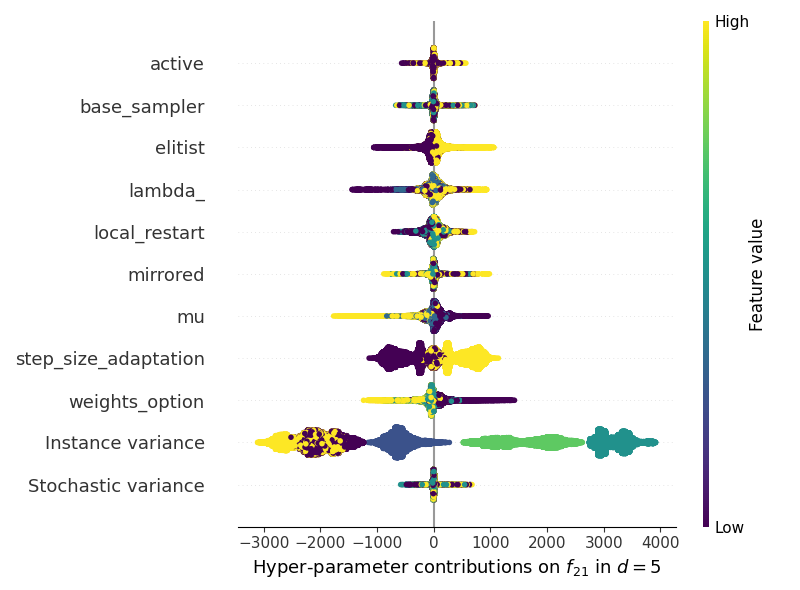
\includegraphics[height=0.15\textheight,trim=0mm 0mm 30mm 0mm,clip]{cma_img_new/img_summary_f21_d5.png}
	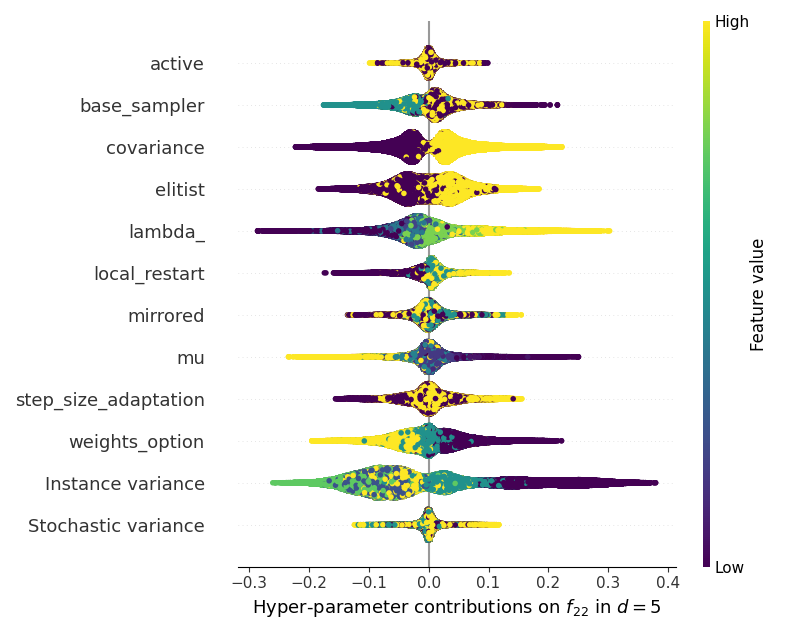
\includegraphics[height=0.15\textheight,trim=60mm 0mm 30mm 0mm,clip]{cma_img_new/img_summary_f22_d5.png}
	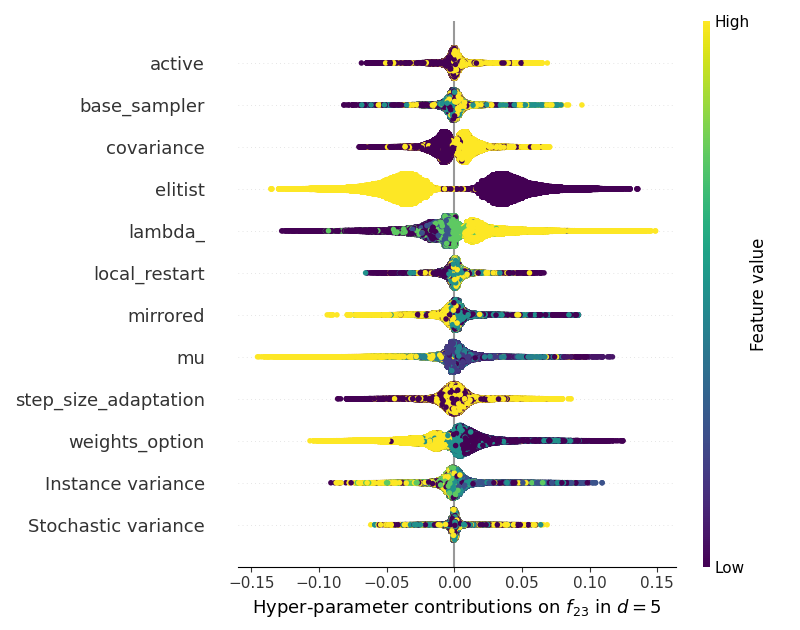
\includegraphics[height=0.15\textheight,trim=60mm 0mm 30mm 0mm,clip]{cma_img_new/img_summary_f23_d5.png}
	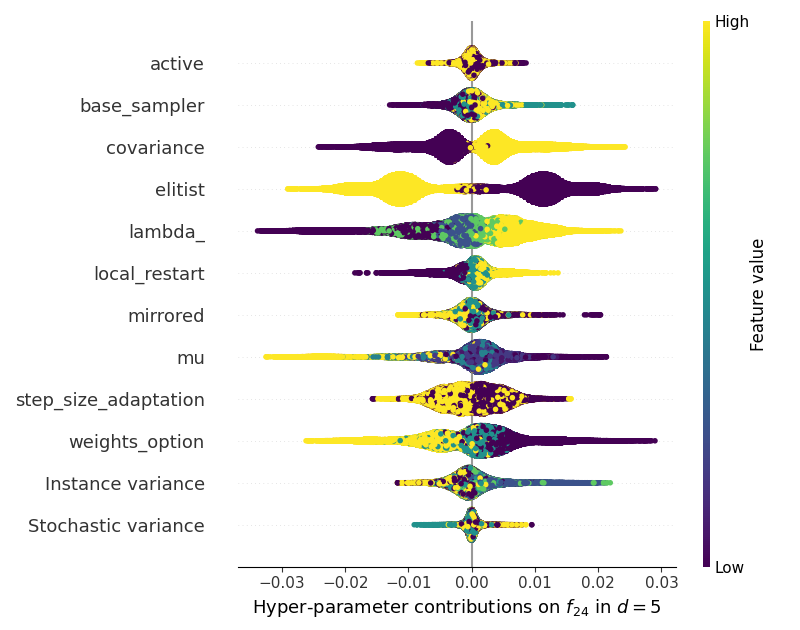
\includegraphics[height=0.15\textheight,trim=60mm 0mm 0mm 0mm,clip]{cma_img_new/img_summary_f24_d5.png}
\caption{Hyper-parameter contributions per benchmark function for d=5. \label{fig:shapxplaind5}}

\end{figure}

\begin{figure}[t]
\centering
	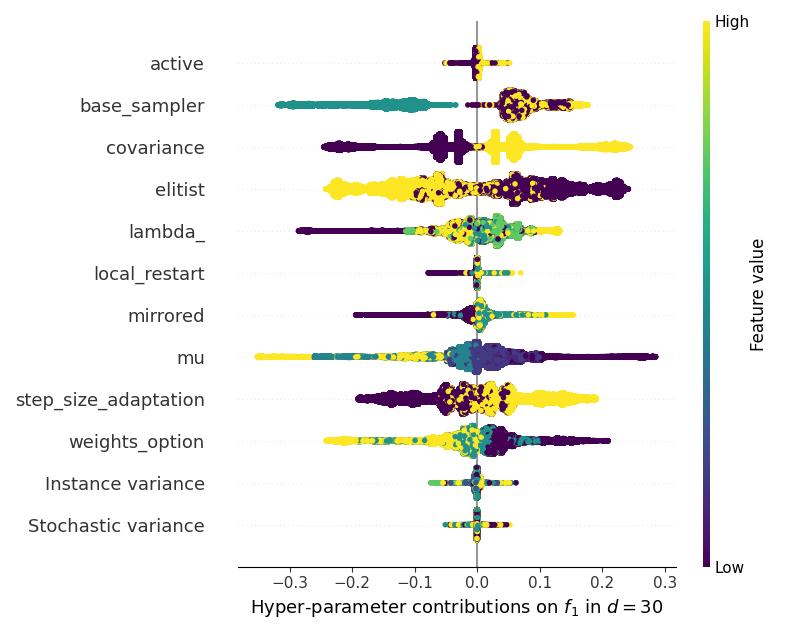
\includegraphics[height=0.15\textheight,trim=0mm 0mm 30mm 0mm,clip]{cma_img_new/img_summary_f1_d30.png}
	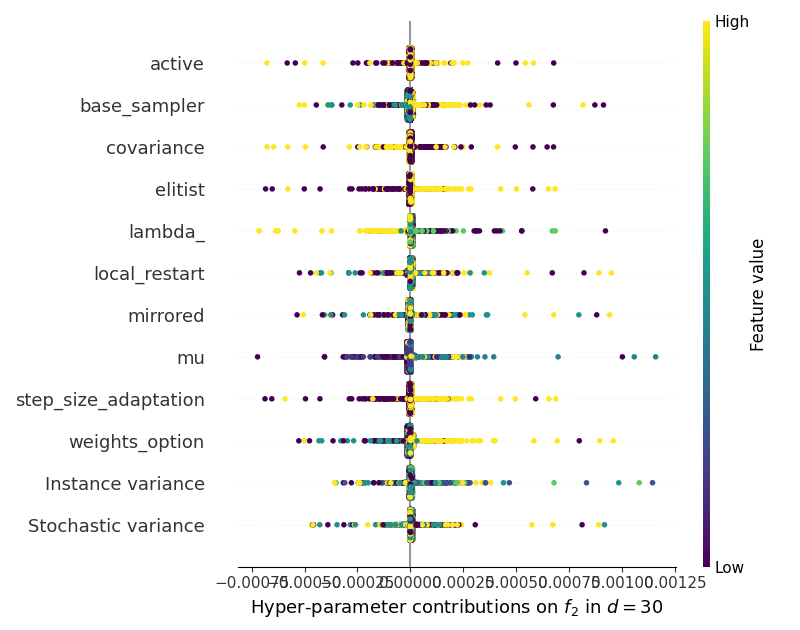
\includegraphics[height=0.15\textheight,trim=60mm 0mm 30mm 0mm,clip]{cma_img_new/img_summary_f2_d30.png}
	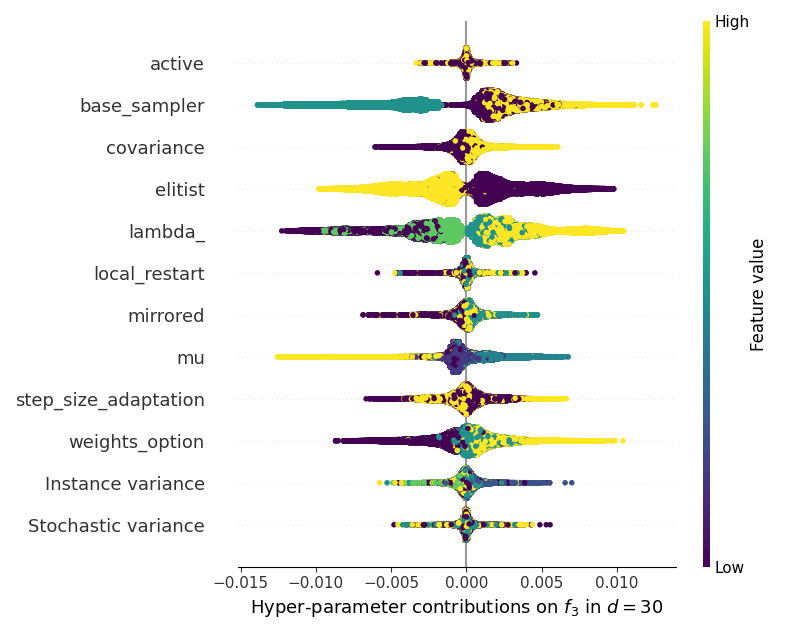
\includegraphics[height=0.15\textheight,trim=60mm 0mm 30mm 0mm,clip]{cma_img_new/img_summary_f3_d30.png}
	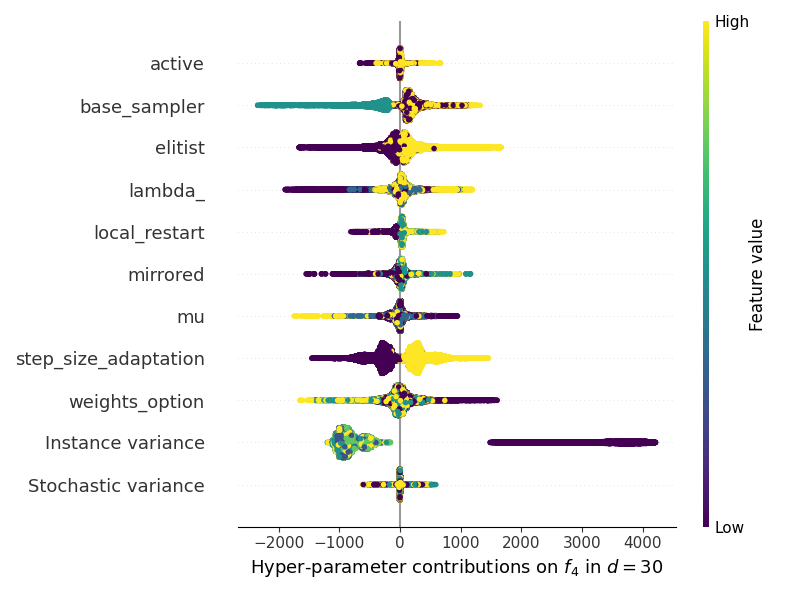
\includegraphics[height=0.15\textheight,trim=60mm 0mm 0mm 0mm,clip]{cma_img_new/img_summary_f4_d30.png}
	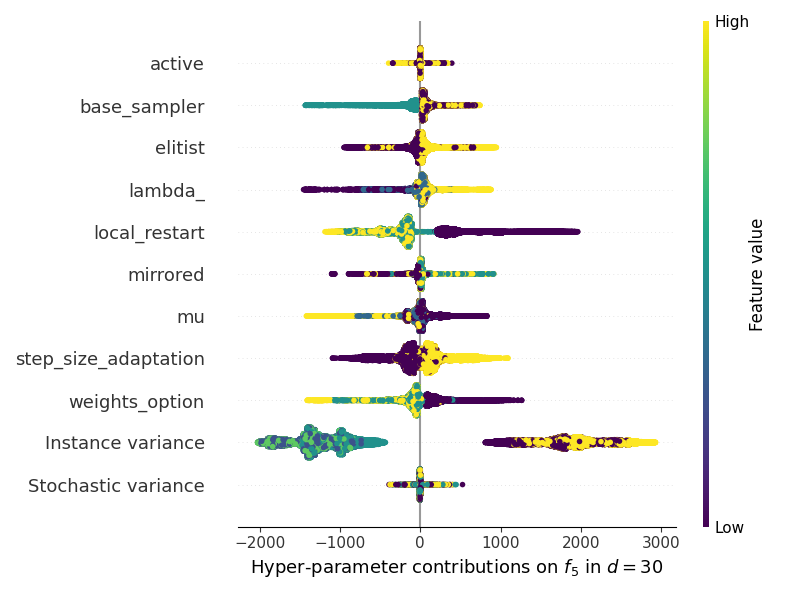
\includegraphics[height=0.15\textheight,trim=0mm 0mm 30mm 0mm,clip]{cma_img_new/img_summary_f5_d30.png}
	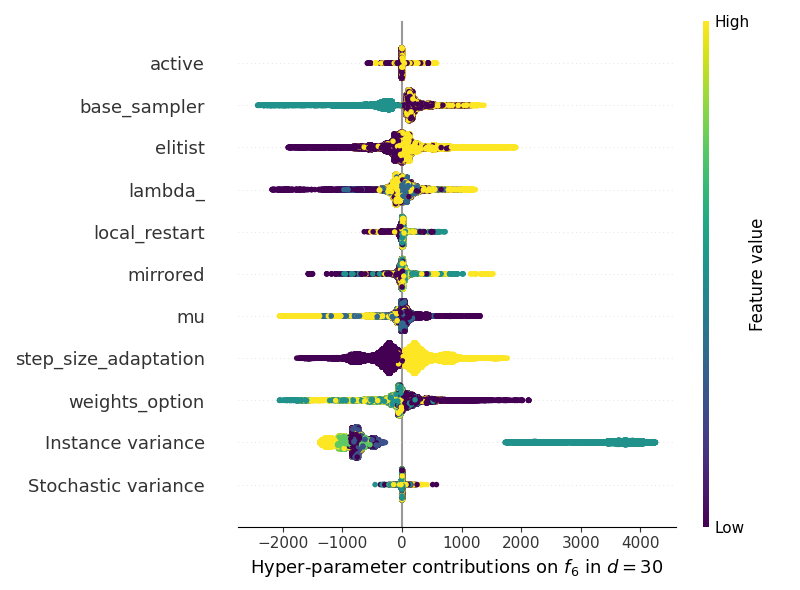
\includegraphics[height=0.15\textheight,trim=60mm 0mm 30mm 0mm,clip]{cma_img_new/img_summary_f6_d30.png}
	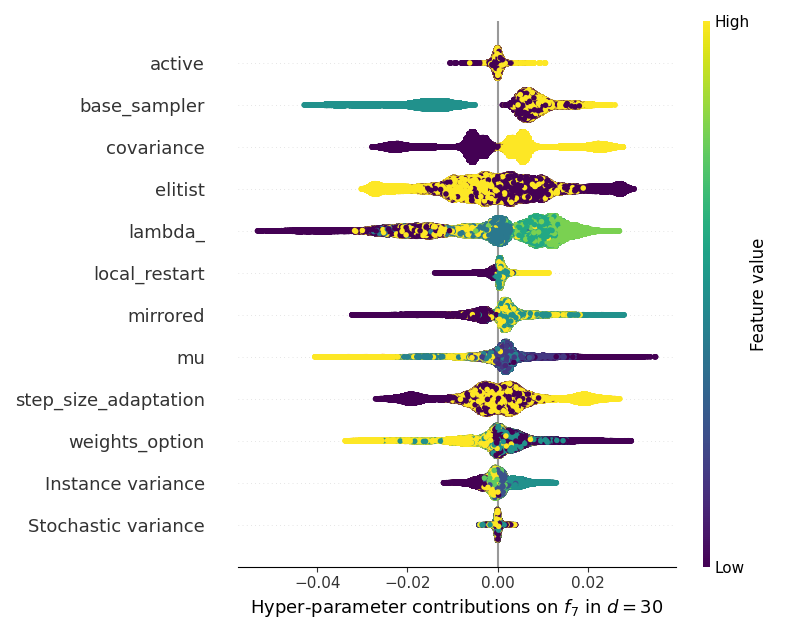
\includegraphics[height=0.15\textheight,trim=60mm 0mm 30mm 0mm,clip]{cma_img_new/img_summary_f7_d30.png}
	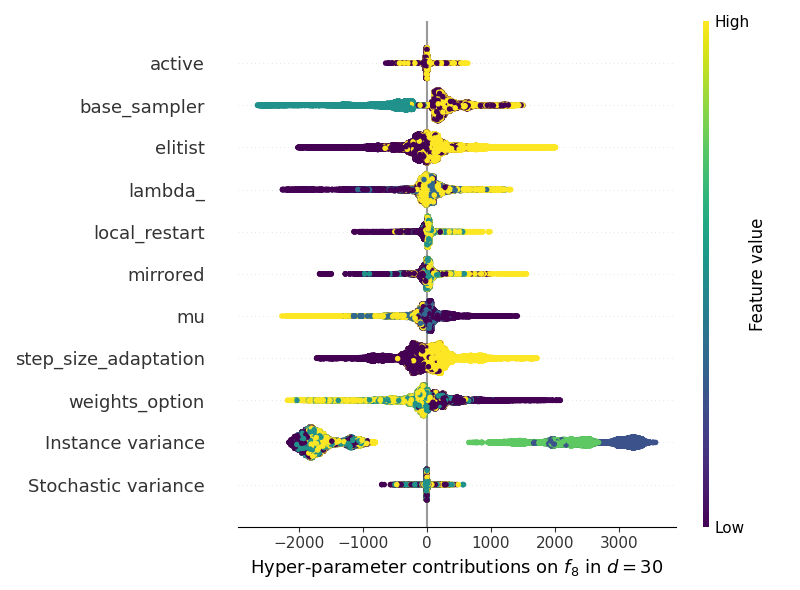
\includegraphics[height=0.15\textheight,trim=60mm 0mm 0mm 0mm,clip]{cma_img_new/img_summary_f8_d30.png}
	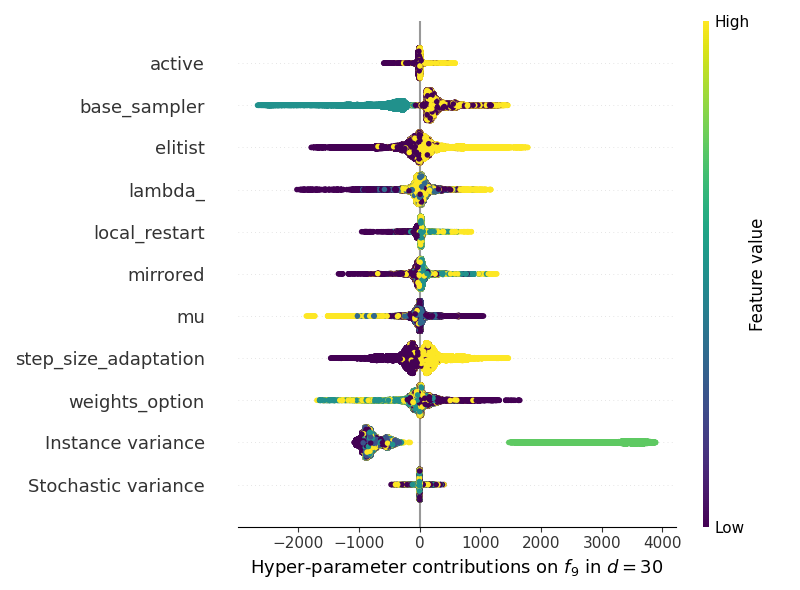
\includegraphics[height=0.15\textheight,trim=0mm 0mm 30mm 0mm,clip]{cma_img_new/img_summary_f9_d30.png}
	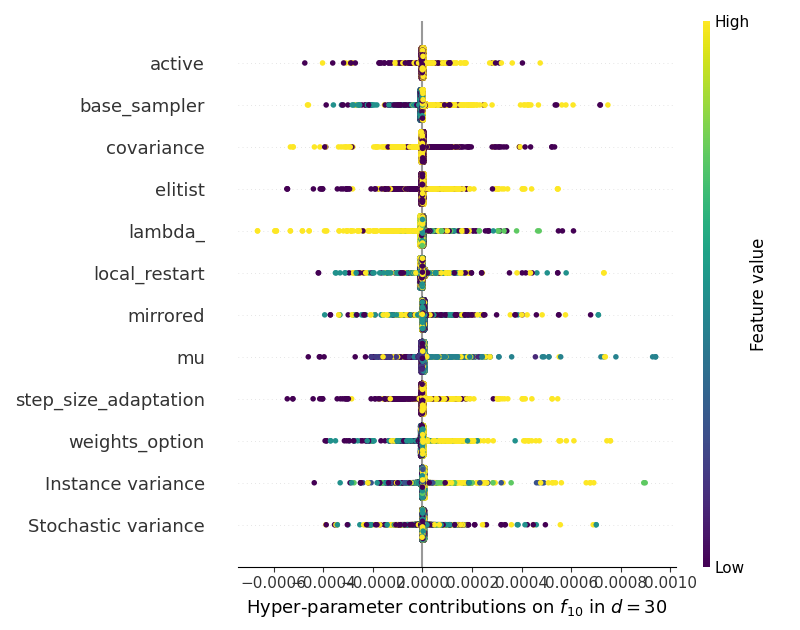
\includegraphics[height=0.15\textheight,trim=60mm 0mm 30mm 0mm,clip]{cma_img_new/img_summary_f10_d30.png}
	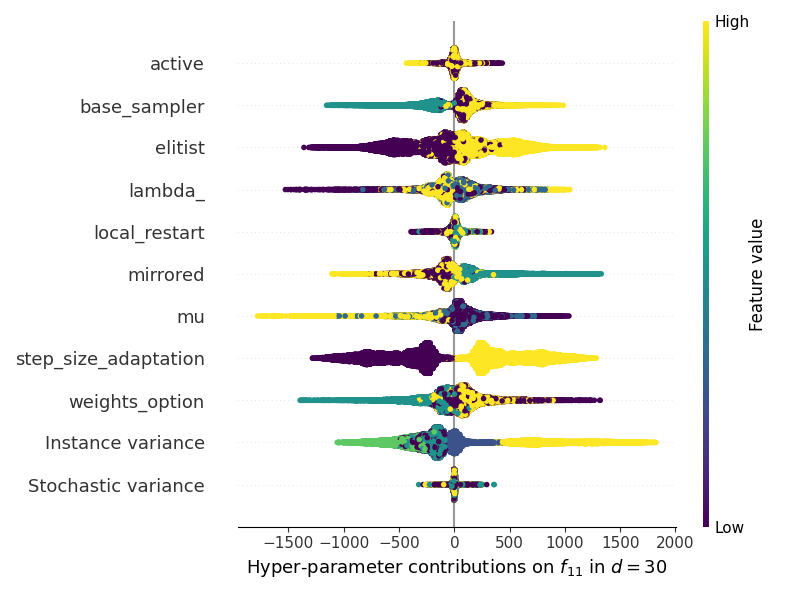
\includegraphics[height=0.15\textheight,trim=60mm 0mm 30mm 0mm,clip]{cma_img_new/img_summary_f11_d30.png}
	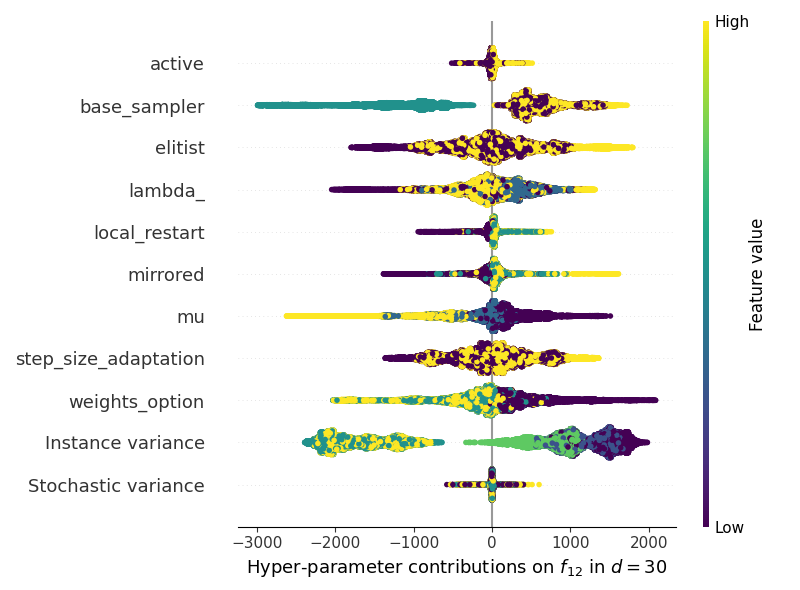
\includegraphics[height=0.15\textheight,trim=60mm 0mm 0mm 0mm,clip]{cma_img_new/img_summary_f12_d30.png}
	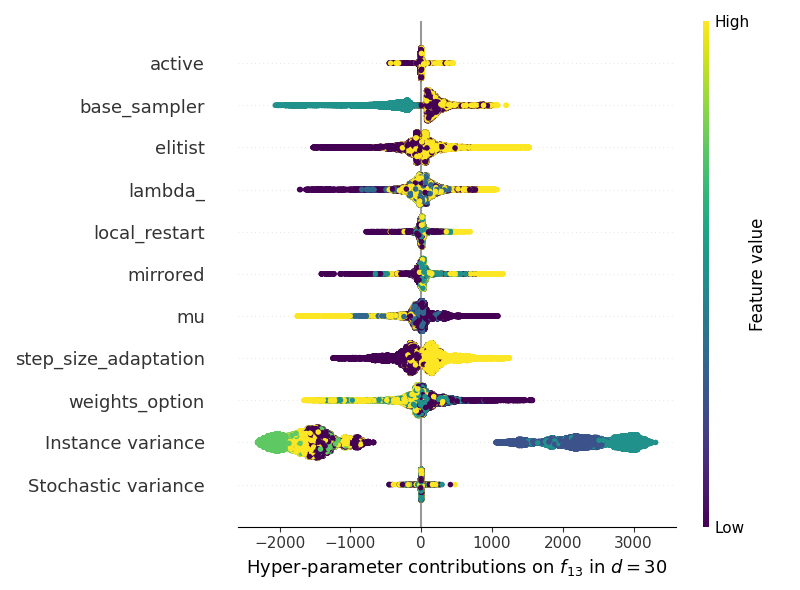
\includegraphics[height=0.15\textheight,trim=0mm 0mm 30mm 0mm,clip]{cma_img_new/img_summary_f13_d30.png}
	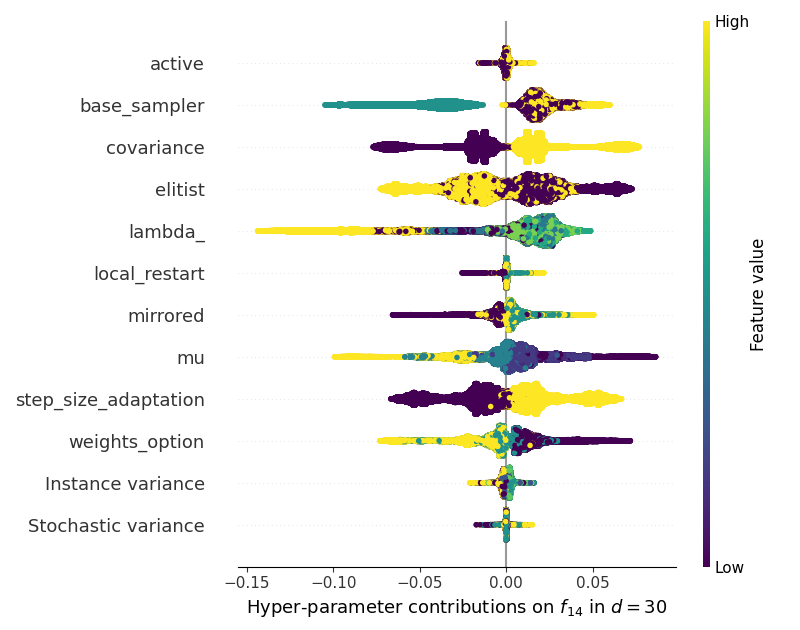
\includegraphics[height=0.15\textheight,trim=60mm 0mm 30mm 0mm,clip]{cma_img_new/img_summary_f14_d30.png}
	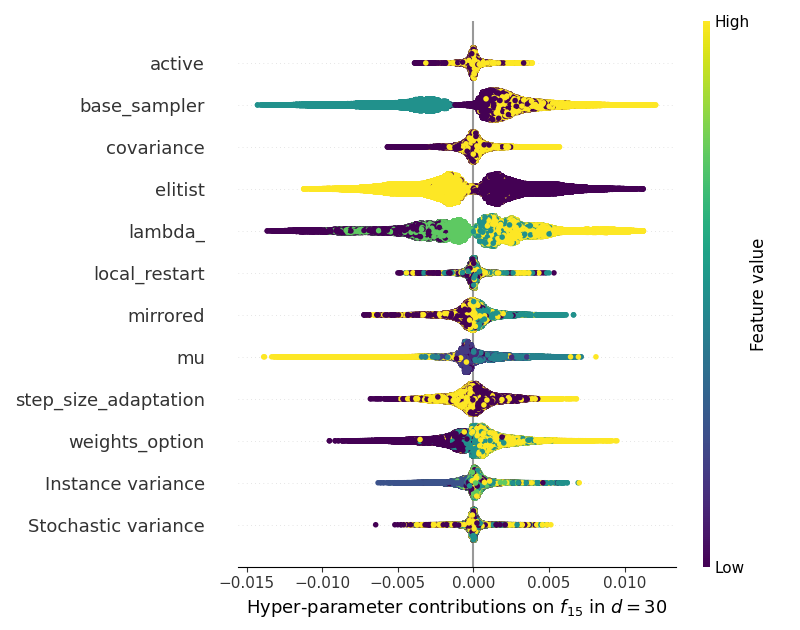
\includegraphics[height=0.15\textheight,trim=60mm 0mm 30mm 0mm,clip]{cma_img_new/img_summary_f15_d30.png}
	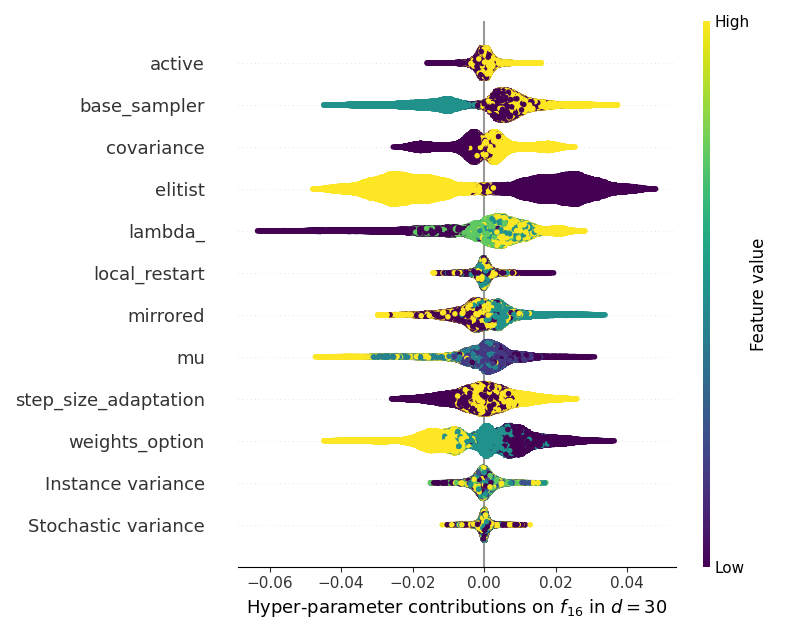
\includegraphics[height=0.15\textheight,trim=60mm 0mm 0mm 0mm,clip]{cma_img_new/img_summary_f16_d30.png}
	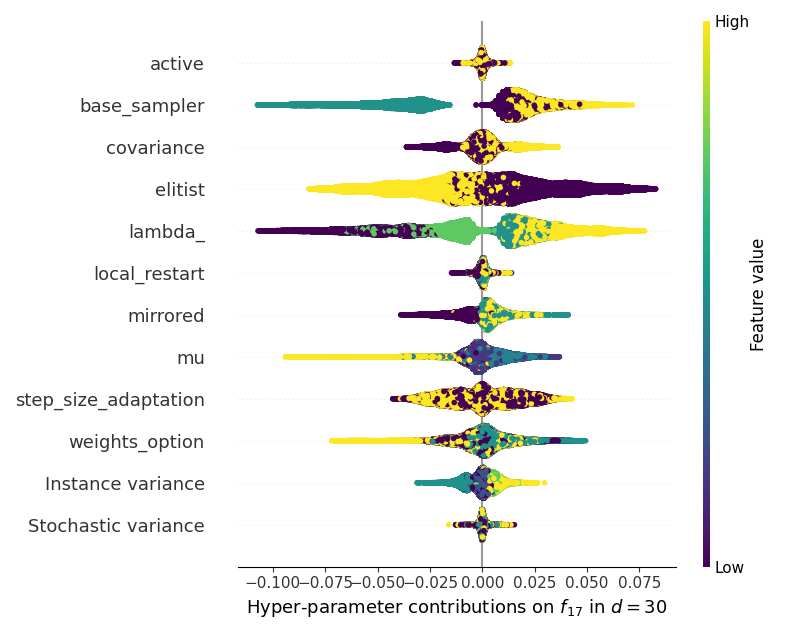
\includegraphics[height=0.15\textheight,trim=0mm 0mm 30mm 0mm,clip]{cma_img_new/img_summary_f17_d30.png}
	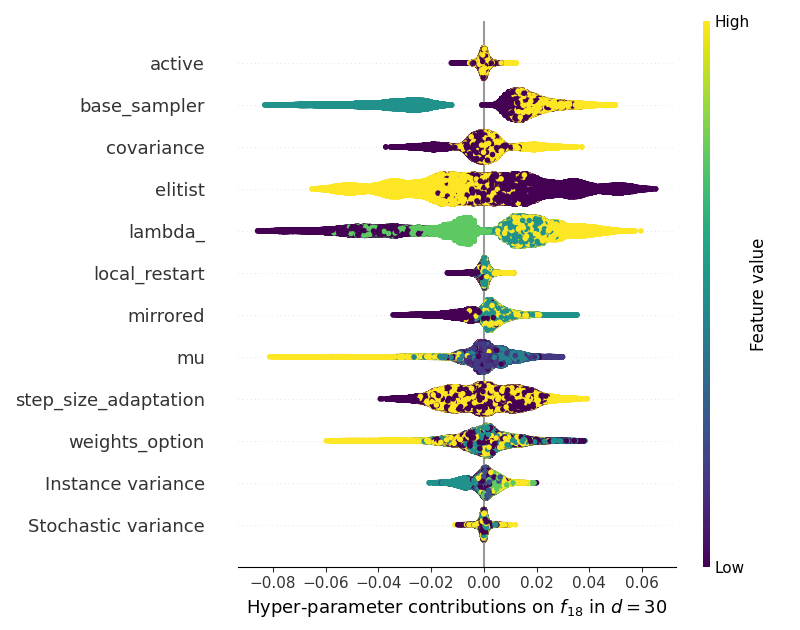
\includegraphics[height=0.15\textheight,trim=60mm 0mm 30mm 0mm,clip]{cma_img_new/img_summary_f18_d30.png}
	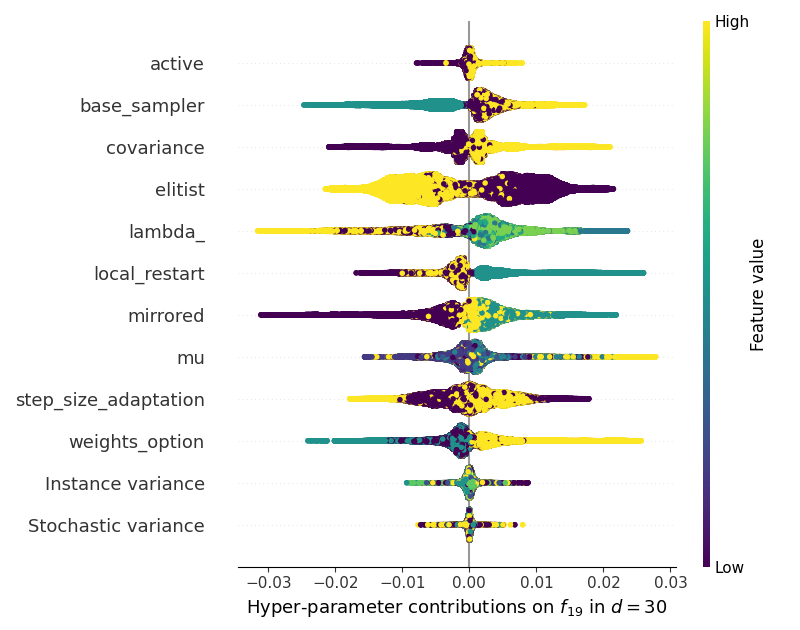
\includegraphics[height=0.15\textheight,trim=60mm 0mm 30mm 0mm,clip]{cma_img_new/img_summary_f19_d30.png}
	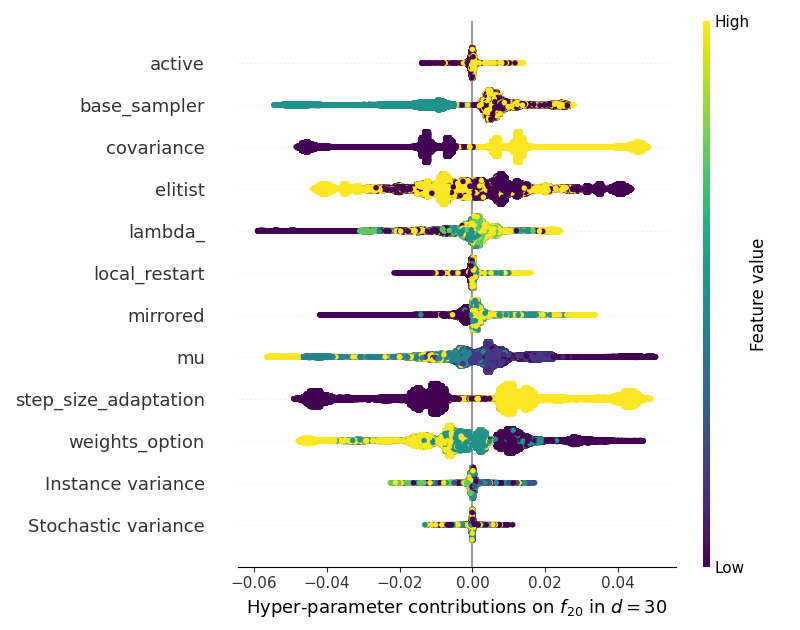
\includegraphics[height=0.15\textheight,trim=60mm 0mm 0mm 0mm,clip]{cma_img_new/img_summary_f20_d30.png}
	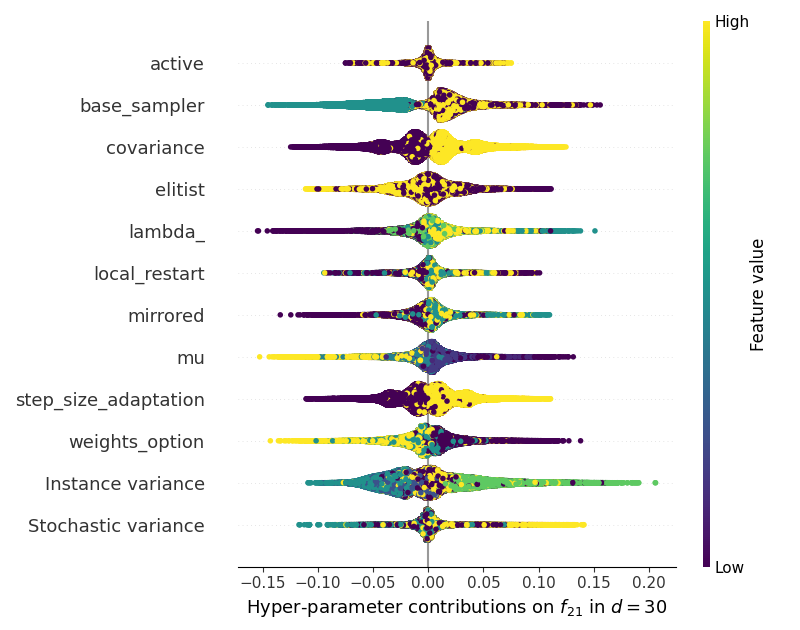
\includegraphics[height=0.15\textheight,trim=0mm 0mm 30mm 0mm,clip]{cma_img_new/img_summary_f21_d30.png}
	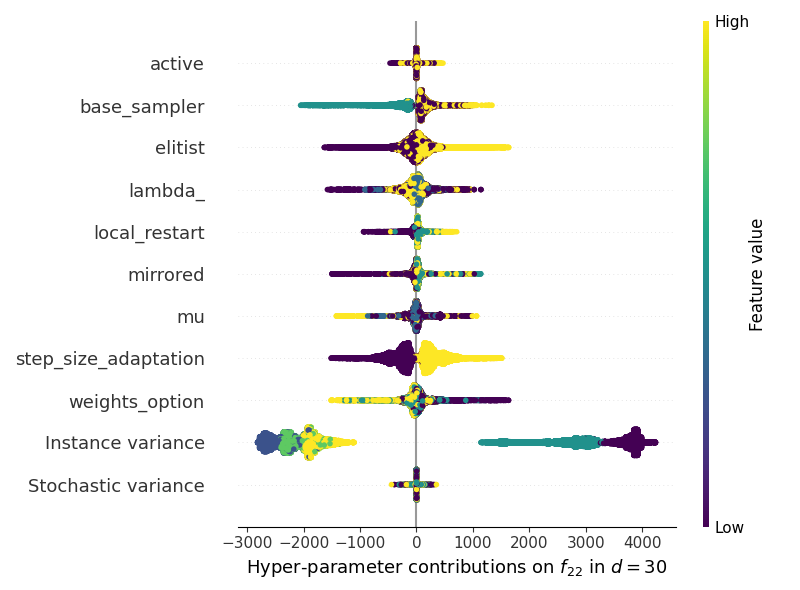
\includegraphics[height=0.15\textheight,trim=60mm 0mm 30mm 0mm,clip]{cma_img_new/img_summary_f22_d30.png}
	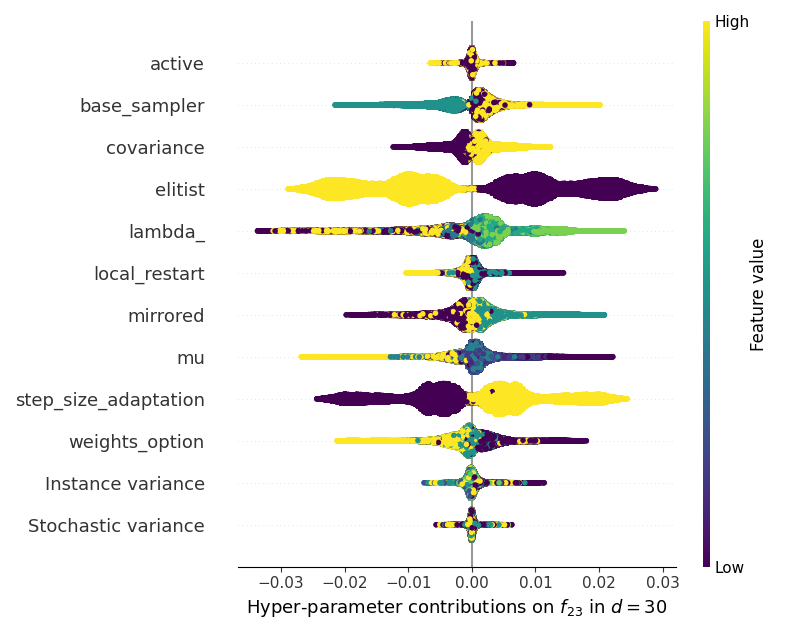
\includegraphics[height=0.15\textheight,trim=60mm 0mm 30mm 0mm,clip]{cma_img_new/img_summary_f23_d30.png}
	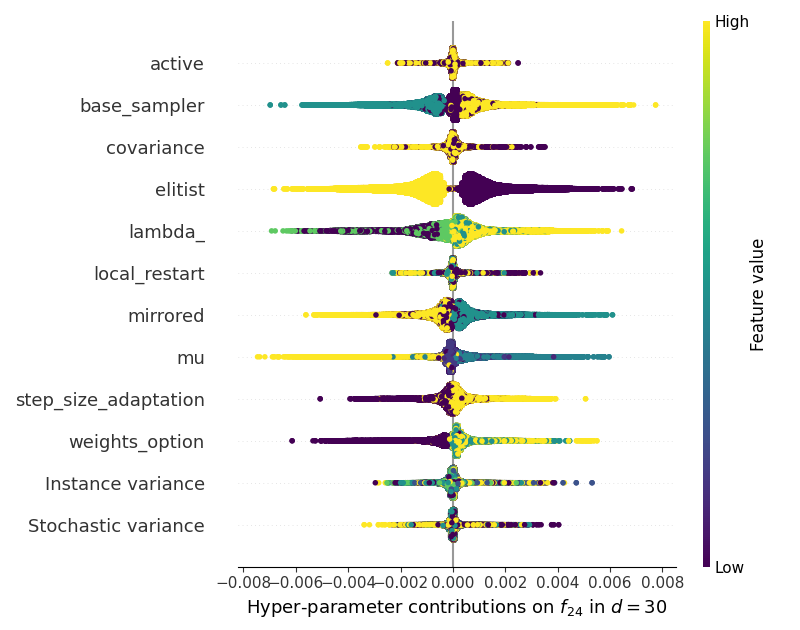
\includegraphics[height=0.15\textheight,trim=60mm 0mm 0mm 0mm,clip]{cma_img_new/img_summary_f24_d30.png}
\caption{Hyper-parameter contributions per benchmark function for d=30. \label{fig:shapxplaind30}}

\end{figure}

% Performance stats per dimension and function for mod-CMA. Boldface for the single-best configuration indicates a significant improvement over the average best configuration (for that dimension), Boldface for the average best configuration indicates a significant improvement over the average AUC of all configurations.
\begin{table}
\caption{Performance of single-best, average best and average algorithm performance over all configurations per function and dimension.}
\begin{tabular}{llllllll}
\toprule
\multicolumn{4}{c}{d=5} & \multicolumn{4}{c}{d=30} \\
Function & single-best & avg-best & all & Function & single-best & avg-best & all \\
\midrule
f1 Sphere & \textbf{0.00 (0.00)} & \textbf{0.00 (0.00)} & 0.00 (0.00) & f1 Sphere & \textbf{0.00 (0.00)} & \textbf{0.00 (0.00)} & 0.00 (0.00) \\
f2 Ellipsoid & \textbf{0.00 (0.00)} & \textbf{0.00 (0.00)} & 0.00 (0.00) & f2 Ellipsoid & 0.00 (0.00) & \textbf{0.00 (0.00)} & 0.00 (0.00) \\
f3 Rastrigin & \textbf{0.00 (0.00)} & \textbf{0.00 (0.00)} & 0.00 (0.00) & f3 Rastrigin & \textbf{0.00 (0.00)} & \textbf{0.00 (0.00)} & 0.00 (0.00) \\
f4 BuecheRastrigin & \textbf{0.00 (0.00)} & \textbf{0.00 (0.00)} & 0.00 (0.00) & f4 BuecheRastrigin & \textbf{0.00 (0.00)} & \textbf{0.00 (0.00)} & 0.00 (0.00) \\
f5 LinearSlope & \textbf{0.00 (0.00)} & 0.00 (0.00) & 0.00 (0.00) & f5 LinearSlope & \textbf{0.00 (0.00)} & 0.00 (0.00) & 0.00 (0.00) \\
f6 AttractiveSector & \textbf{0.00 (0.00)} & \textbf{0.00 (0.00)} & 0.00 (0.00) & f6 AttractiveSector & 0.00 (0.00) & \textbf{0.00 (0.00)} & 0.00 (0.00) \\
f7 StepEllipsoid & \textbf{0.00 (0.00)} & \textbf{0.00 (0.00)} & 0.00 (0.00) & f7 StepEllipsoid & 0.00 (0.00) & \textbf{0.00 (0.00)} & 0.00 (0.00) \\
f8 Rosenbrock & \textbf{0.00 (0.00)} & \textbf{0.00 (0.00)} & 0.00 (0.00) & f8 Rosenbrock & 0.00 (0.00) & \textbf{0.00 (0.00)} & 0.00 (0.00) \\
f9 RosenbrockRotated & \textbf{0.00 (0.00)} & \textbf{0.00 (0.00)} & 0.00 (0.00) & f9 RosenbrockRotated & 0.00 (0.00) & \textbf{0.00 (0.00)} & 0.00 (0.00) \\
f10 EllipsoidRotated & \textbf{0.00 (0.00)} & \textbf{0.00 (0.00)} & 0.00 (0.00) & f10 EllipsoidRotated & 0.00 (0.00) & \textbf{0.00 (0.00)} & 0.00 (0.00) \\
f11 Discus & 0.00 (0.00) & \textbf{0.00 (0.00)} & 0.00 (0.00) & f11 Discus & 0.00 (0.00) & \textbf{0.00 (0.00)} & 0.00 (0.00) \\
f12 BentCigar & \textbf{0.00 (0.00)} & \textbf{0.00 (0.00)} & 0.00 (0.00) & f12 BentCigar & 0.00 (0.00) & \textbf{0.00 (0.00)} & 0.00 (0.00) \\
f13 SharpRidge & \textbf{0.00 (0.00)} & \textbf{0.00 (0.00)} & 0.00 (0.00) & f13 SharpRidge & 0.00 (0.00) & \textbf{0.00 (0.00)} & 0.00 (0.00) \\
f14 DifferentPowers & 0.00 (0.00) & \textbf{0.00 (0.00)} & 0.00 (0.00) & f14 DifferentPowers & \textbf{0.00 (0.00)} & \textbf{0.00 (0.00)} & 0.00 (0.00) \\
f15 RastriginRotated & 0.00 (0.00) & \textbf{0.00 (0.00)} & 0.00 (0.00) & f15 RastriginRotated & \textbf{0.00 (0.00)} & \textbf{0.00 (0.00)} & 0.00 (0.00) \\
f16 Weierstrass & \textbf{0.00 (0.00)} & \textbf{0.00 (0.00)} & 0.00 (0.00) & f16 Weierstrass & 0.00 (0.00) & \textbf{0.00 (0.00)} & 0.00 (0.00) \\
f17 Schaffers10 & 0.00 (0.00) & \textbf{0.00 (0.00)} & 0.00 (0.00) & f17 Schaffers10 & \textbf{0.00 (0.00)} & \textbf{0.00 (0.00)} & 0.00 (0.00) \\
f18 Schaffers1000 & 0.00 (0.00) & \textbf{0.00 (0.00)} & 0.00 (0.00) & f18 Schaffers1000 & \textbf{0.00 (0.00)} & \textbf{0.00 (0.00)} & 0.00 (0.00) \\
f19 GriewankRosenbrock & \textbf{0.00 (0.00)} & \textbf{0.00 (0.00)} & 0.00 (0.00) & f19 GriewankRosenbrock & \textbf{0.00 (0.00)} & \textbf{0.00 (0.00)} & 0.00 (0.00) \\
f20 Schwefel & \textbf{0.00 (0.00)} & 0.00 (0.00) & 0.00 (0.00) & f20 Schwefel & \textbf{0.00 (0.00)} & \textbf{0.00 (0.00)} & 0.00 (0.00) \\
f21 Gallagher101 & \textbf{0.00 (0.00)} & 0.00 (0.00) & 0.00 (0.00) & f21 Gallagher101 & 0.00 (0.00) & \textbf{0.00 (0.00)} & 0.00 (0.00) \\
f22 Gallagher21 & 0.00 (0.00) & \textbf{0.00 (0.00)} & 0.00 (0.00) & f22 Gallagher21 & \textbf{0.00 (0.00)} & 0.00 (0.00) & 0.00 (0.00) \\
f23 Katsuura & \textbf{0.00 (0.00)} & \textbf{0.00 (0.00)} & 0.00 (0.00) & f23 Katsuura & \textbf{0.00 (0.00)} & \textbf{0.00 (0.00)} & 0.00 (0.00) \\
f24 LunacekBiRastrigin & \textbf{0.00 (0.00)} & \textbf{0.00 (0.00)} & 0.00 (0.00) & f24 LunacekBiRastrigin & 0.00 (0.00) & \textbf{0.00 (0.00)} & 0.00 (0.00) \\
\bottomrule
\end{tabular}
\end{table}
% Behaviour stats per dimension and function for mod-CMA
\begin{table}
\caption{Algorithm stability of mod-CMA}
\begin{tabular}{lrlr}
\toprule
\multicolumn{2}{c}{d=5} & \multicolumn{2}{c}{d=30} \\
Measure & value & Measure & value \\
\midrule
Algorithm stability & 1.00 & Algorithm stability & 1.00 \\
Invar. avg. best & 1.00 & Invar. avg. best & 1.00 \\
S-inv. avg. best & 1.00 & S-inv. avg. best & 1.00 \\
I-inv. avg. best & 1.00 & I-inv. avg. best & 1.00 \\
Invar. single best & 1.00 & Invar. single best & 1.00 \\
S-inv. single best & 1.00 & S-inv. single best & 1.00 \\
I-inv. single best & 1.00 & I-inv. single best & 1.00 \\
Average norm. perf. & 0.00 & Average norm. perf. & 0.00 \\
Gain avg. best & 0.00 & Gain avg. best & 0.00 \\
Gain single best & 0.00 & Gain single best & 0.00 \\
sig. impr. avg best & 1.00 & sig. impr. avg best & 1.00 \\
sig. impr. s. best vs avg best & 1.00 & sig. impr. s. best vs avg best & 0.00 \\
\bottomrule
\end{tabular}
\end{table}
